\PassOptionsToPackage{unicode=true}{hyperref} % options for packages loaded elsewhere
\PassOptionsToPackage{hyphens}{url}
%
\documentclass[
  ignorenonframetext,
]{beamer}
\usepackage{pgfpages}
\setbeamertemplate{caption}[numbered]
\setbeamertemplate{caption label separator}{: }
\setbeamercolor{caption name}{fg=normal text.fg}
\beamertemplatenavigationsymbolsempty
% Prevent slide breaks in the middle of a paragraph:
\widowpenalties 1 10000
\raggedbottom
\setbeamertemplate{part page}{
  \centering
  \begin{beamercolorbox}[sep=16pt,center]{part title}
    \usebeamerfont{part title}\insertpart\par
  \end{beamercolorbox}
}
\setbeamertemplate{section page}{
  \centering
  \begin{beamercolorbox}[sep=12pt,center]{part title}
    \usebeamerfont{section title}\insertsection\par
  \end{beamercolorbox}
}
\setbeamertemplate{subsection page}{
  \centering
  \begin{beamercolorbox}[sep=8pt,center]{part title}
    \usebeamerfont{subsection title}\insertsubsection\par
  \end{beamercolorbox}
}
\AtBeginPart{
  \frame{\partpage}
}
\AtBeginSection{
  \ifbibliography
  \else
    \frame{\sectionpage}
  \fi
}
\AtBeginSubsection{
  \frame{\subsectionpage}
}
\usepackage{lmodern}
\usepackage{amssymb,amsmath}
\usepackage{ifxetex,ifluatex}
\ifnum 0\ifxetex 1\fi\ifluatex 1\fi=0 % if pdftex
  \usepackage[T1]{fontenc}
  \usepackage[utf8]{inputenc}
  \usepackage{textcomp} % provides euro and other symbols
\else % if luatex or xelatex
  \usepackage{unicode-math}
  \defaultfontfeatures{Scale=MatchLowercase}
  \defaultfontfeatures[\rmfamily]{Ligatures=TeX,Scale=1}
\fi
% use upquote if available, for straight quotes in verbatim environments
\IfFileExists{upquote.sty}{\usepackage{upquote}}{}
\IfFileExists{microtype.sty}{% use microtype if available
  \usepackage[]{microtype}
  \UseMicrotypeSet[protrusion]{basicmath} % disable protrusion for tt fonts
}{}
\makeatletter
\@ifundefined{KOMAClassName}{% if non-KOMA class
  \IfFileExists{parskip.sty}{%
    \usepackage{parskip}
  }{% else
    \setlength{\parindent}{0pt}
    \setlength{\parskip}{6pt plus 2pt minus 1pt}}
}{% if KOMA class
  \KOMAoptions{parskip=half}}
\makeatother
\usepackage{xcolor}
\IfFileExists{xurl.sty}{\usepackage{xurl}}{} % add URL line breaks if available
\IfFileExists{bookmark.sty}{\usepackage{bookmark}}{\usepackage{hyperref}}
\hypersetup{
  pdftitle={Survival analysis in decision modeling},
  pdfauthor={petros.pechlivanoglou@sickkids.ca},
  pdfborder={0 0 0},
  breaklinks=true}
\urlstyle{same}  % don't use monospace font for urls
\newif\ifbibliography
\usepackage{graphicx,grffile}
\makeatletter
\def\maxwidth{\ifdim\Gin@nat@width>\linewidth\linewidth\else\Gin@nat@width\fi}
\def\maxheight{\ifdim\Gin@nat@height>\textheight\textheight\else\Gin@nat@height\fi}
\makeatother
% Scale images if necessary, so that they will not overflow the page
% margins by default, and it is still possible to overwrite the defaults
% using explicit options in \includegraphics[width, height, ...]{}
\setkeys{Gin}{width=\maxwidth,height=\maxheight,keepaspectratio}
\setlength{\emergencystretch}{3em}  % prevent overfull lines
\providecommand{\tightlist}{%
  \setlength{\itemsep}{0pt}\setlength{\parskip}{0pt}}
\setcounter{secnumdepth}{-2}

% set default figure placement to htbp
\makeatletter
\def\fps@figure{htbp}
\makeatother


\title{Survival analysis in decision modeling}
\subtitle{The DARTH Workgroup}
\author{\href{mailto:petros.pechlivanoglou@sickkids.ca}{\nolinkurl{petros.pechlivanoglou@sickkids.ca}}}
\date{10/16/2019}

\begin{document}
\frame{\titlepage}

\begin{frame}{Overview}
\protect\hypertarget{overview}{}

\begin{itemize}
\tightlist
\item
  Motivation and introduction in Survival analysis
\item
  Survival modeling
\item
  Partitioned survival modeling
\item
  Multistate models
\item
  Advanced topiics

  \begin{itemize}
  \tightlist
  \item
    Mixture cure models
  \item
    External evidence in survival models
  \end{itemize}
\end{itemize}

\end{frame}

\begin{frame}{It's all about the data!}
\protect\hypertarget{its-all-about-the-data}{}

\begin{itemize}
\tightlist
\item
  RCT evidence often not sufficient for Health Technology Assesment
  (HTA)

  \begin{itemize}
  \tightlist
  \item
    Short follow up
  \item
    Patients lost during follow up
  \item
    Often not reflective of real world
  \item
    Right skewed\\
  \item
    Information ``flowing'' over intervals
  \item
    Extrapolation often necessary
  \end{itemize}
\end{itemize}

\end{frame}

\begin{frame}{Bonus challenges in Oncology RCTs}
\protect\hypertarget{bonus-challenges-in-oncology-rcts}{}

\begin{itemize}
\tightlist
\item
  Overall Survival (OS), Progression-Free Survival (PFS)
\item
  Trials powered to show differences on PFS and not OS
\item
  Cross-over
\item
  PFS and OS data are correlated
\item
  Access to patient level OS data not always the case
\end{itemize}

\end{frame}

\begin{frame}{Censoring}
\protect\hypertarget{censoring}{}

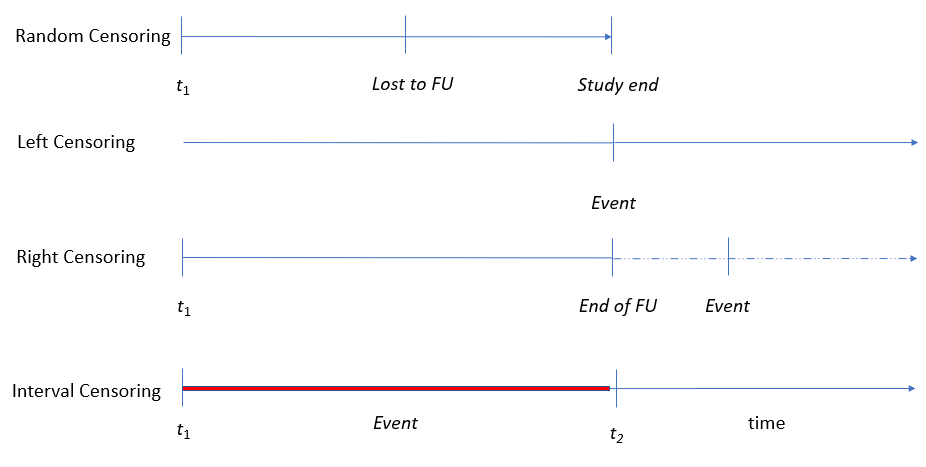
\includegraphics[width=1\linewidth]{figures/censoring}

\end{frame}

\begin{frame}{What is survival analysis}
\protect\hypertarget{what-is-survival-analysis}{}

\begin{itemize}
\item
  Set of statistical methods that can handle:

  \begin{itemize}
  \tightlist
  \item
    Data skewness
  \item
    Censoring
  \item
    (Time-dependent) Covariates
  \item
    State transition processes
  \item
    Recurrent events
  \item
    The expectation of cure
  \end{itemize}
\item
  Used for both inference and extrapolation
\item
  Survival: the probability of not experiencing an event unit some time
  \(t\)
\end{itemize}

\(S(t) = Pr(T >t) = 1- Pr(T \leq t)\)

\end{frame}

\begin{frame}{Types of survival analysis models}
\protect\hypertarget{types-of-survival-analysis-models}{}

\begin{itemize}
\tightlist
\item
  Non-parametric models (e.g.~Kaplan Meier)
\item
  Semi-Parametric models (e.g.~Cox Proportional Hazard)
\item
  Parametric models (e.g.~Accelerated Failure Time)
\end{itemize}

\end{frame}

\begin{frame}{Non-Parametric models}
\protect\hypertarget{non-parametric-models}{}

\begin{itemize}
\tightlist
\item
  Kaplan Meier curves
\end{itemize}

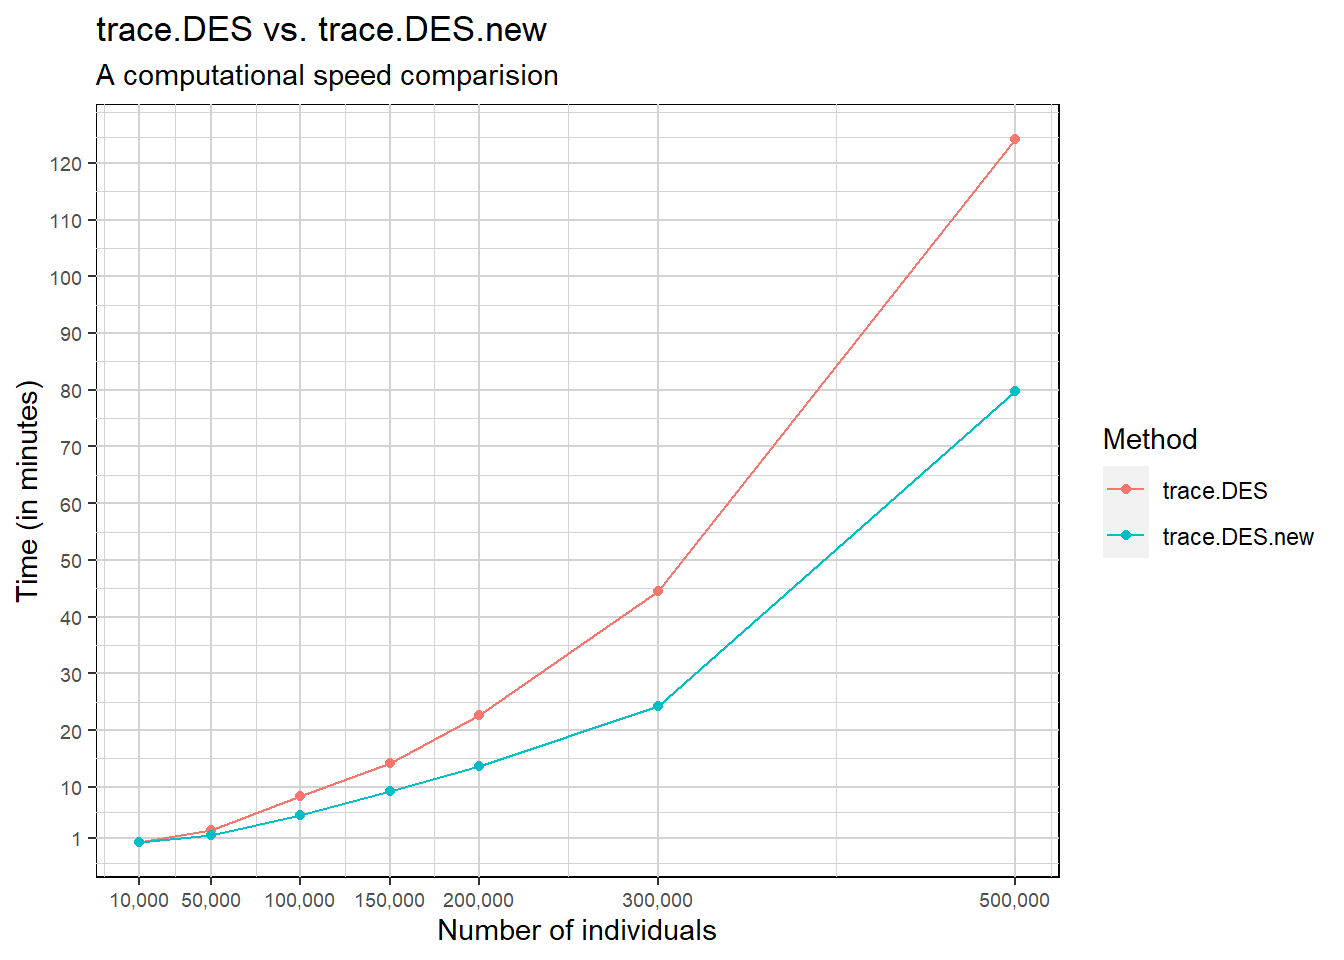
\includegraphics[width=1\linewidth]{SMDM_surv_files/figure-beamer/unnamed-chunk-2-1}

\end{frame}

\begin{frame}

\begin{itemize}
\tightlist
\item
  Nelson Aalen cumulative hazard
\end{itemize}

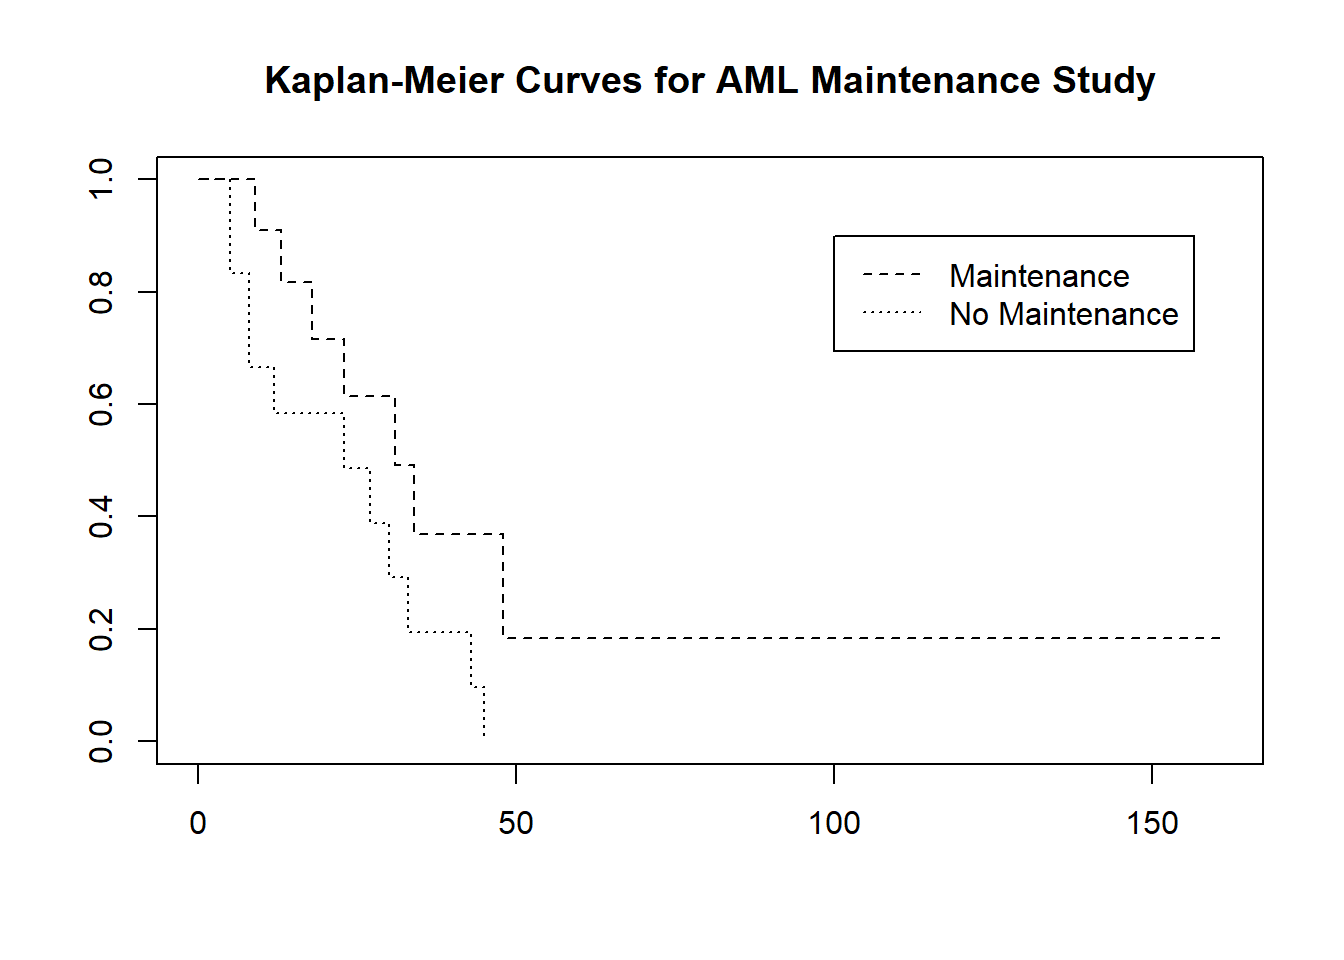
\includegraphics[width=1\linewidth]{SMDM_surv_files/figure-beamer/unnamed-chunk-3-1}

\end{frame}

\begin{frame}{Semi- Parametric models}
\protect\hypertarget{semi--parametric-models}{}

\begin{itemize}
\tightlist
\item
  Cox proportional hazard model

  \begin{itemize}
  \tightlist
  \item
    Hazard: the instantaneous risk of an event at time \(t\),
    conditional on survival to that time.
  \end{itemize}
\item
  Semi:

  \begin{itemize}
  \tightlist
  \item
    Baseline hazard modelled non parametrically (i.e effect of time)
  \item
    Covariate effects ( \(\beta\) 's) modelled parametrically (like in a
    regression model)
  \end{itemize}
\end{itemize}

\end{frame}

\begin{frame}{Fully Parametric models}
\protect\hypertarget{fully-parametric-models}{}

\begin{itemize}
\tightlist
\item
  Usually model time-to-event directly rather than hazard
\item
  Resemble a regression model but can capture censoring
\item
  Fit a distribution to the (observed) time-to-event data

  \begin{itemize}
  \tightlist
  \item
    1 parameter : exponential
  \item
    2 parameter : Weibull, lognormal, gamma etc
  \item
    3, 4 parameter: Gen.~gamma , Gen F etc
  \end{itemize}
\item
  Assumption that censored patients will follow similar patterns to the
  observed.
\item
  Temporal extrapolation possible !
\end{itemize}

\end{frame}

\begin{frame}{Choosing the ``right'' distribution}
\protect\hypertarget{choosing-the-right-distribution}{}

\begin{itemize}
\tightlist
\item
  Statistical considerations of goodness-of-fit
\item
  Clinical plausibility

  \begin{itemize}
  \tightlist
  \item
    in-sample
  \item
    extrapolations
  \item
    out-of-sample
  \end{itemize}
\end{itemize}

\end{frame}

\begin{frame}{Goodness of fit metrics}
\protect\hypertarget{goodness-of-fit-metrics}{}

\begin{itemize}
\item
  Likelihood based metrics
\item
  Akaike Information Criterion (AIC)
\item
  Bayesian Information Criterion (BIC)
\item
  Performance based metrics
\item
  Sensitivity , Specificity
\item
  (time dependent) Receiver Operating characteristic (ROC) curve
\item
  Area Under the Curve (AUC)
\item
  c- statistic
\end{itemize}

\end{frame}

\begin{frame}{Choosing the ``right'' distribution}
\protect\hypertarget{choosing-the-right-distribution-1}{}

\begin{itemize}
\tightlist
\item
  NICE Decision Support Unit
\item
  Latimer et al 2011 : Survival Analysis For Economic Evaluations
  Alongside Clinical Trials - Extrapolation with Patient-Level Data

  \begin{itemize}
  \tightlist
  \item
    \textbf{Survival Model Selection Process algorithm}:

    \begin{itemize}
    \tightlist
    \item
      \emph{recommendations for how survival analysis can be undertaken
      more systematically. This involves fitting and testing a range of
      survival models and comparing these based upon internal validity
      (how well they fit to the observed trial data) and external
      validity (how plausible their extrapolated portions are)}
    \end{itemize}
  \end{itemize}
\end{itemize}

\end{frame}

\begin{frame}{Choosing the ``right'' distribution}
\protect\hypertarget{choosing-the-right-distribution-2}{}

Latimer et al 2011 (DSU 14)

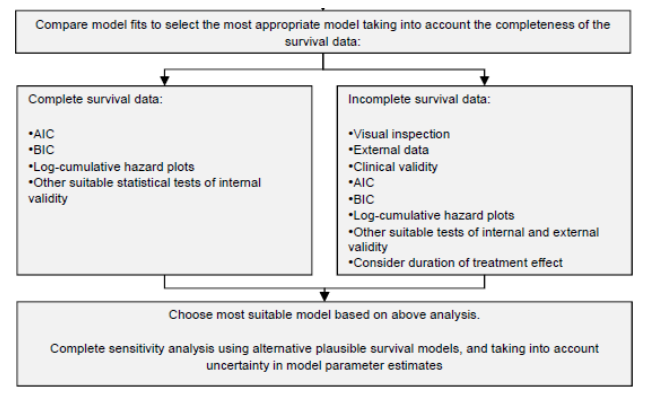
\includegraphics[width=1\linewidth]{figures/goflatimer}

\end{frame}

\begin{frame}{Flexible Survival models}
\protect\hypertarget{flexible-survival-models}{}

\begin{itemize}
\tightlist
\item
  Multi - parameter distributions

  \begin{itemize}
  \tightlist
  \item
    Generalized Gamma
  \item
    Generalized F
  \item
    Data hungry - possibiliy of overfitting\\
  \item
    Hypothesis testing possible
  \end{itemize}
\end{itemize}

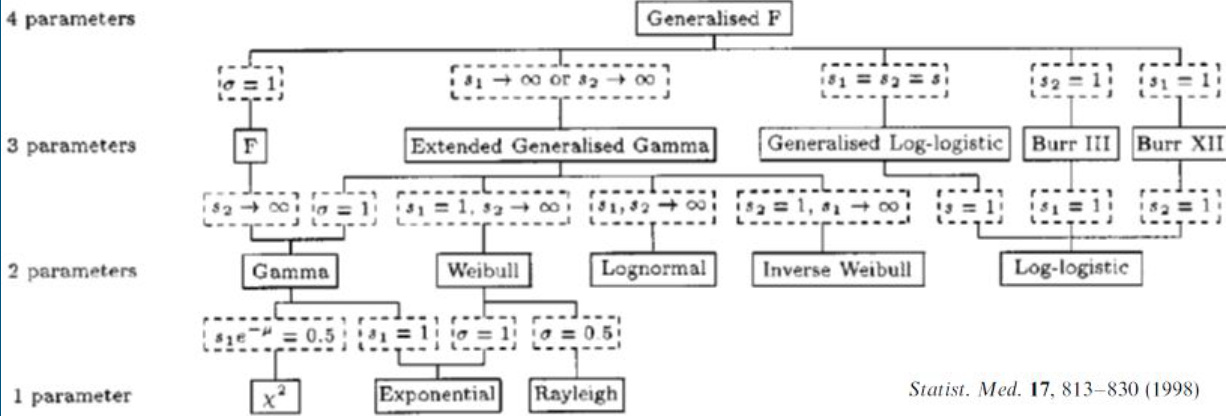
\includegraphics[width=1\linewidth]{figures/genf}

\end{frame}

\begin{frame}{Spline Survival models}
\protect\hypertarget{spline-survival-models}{}

\begin{itemize}
\tightlist
\item
  Survival models where the underlying hazard of an event is modelled as
  a smooth, piecewise polynomial function of time.
\item
  Extrapolation of hazard possible
\item
  Non-linear relation of time and hazard
\item
  Conventionally \emph{knots} are evenly spread on the (log)-time axis
\item
  Overfitting with too many knots possible -sensitivity analysis
\item
  AIC, BIC valid GoF tests
\end{itemize}

\end{frame}

\begin{frame}{Spline Survival models}
\protect\hypertarget{spline-survival-models-1}{}

Gibson et al (Pharmacoeconomics, 2017)

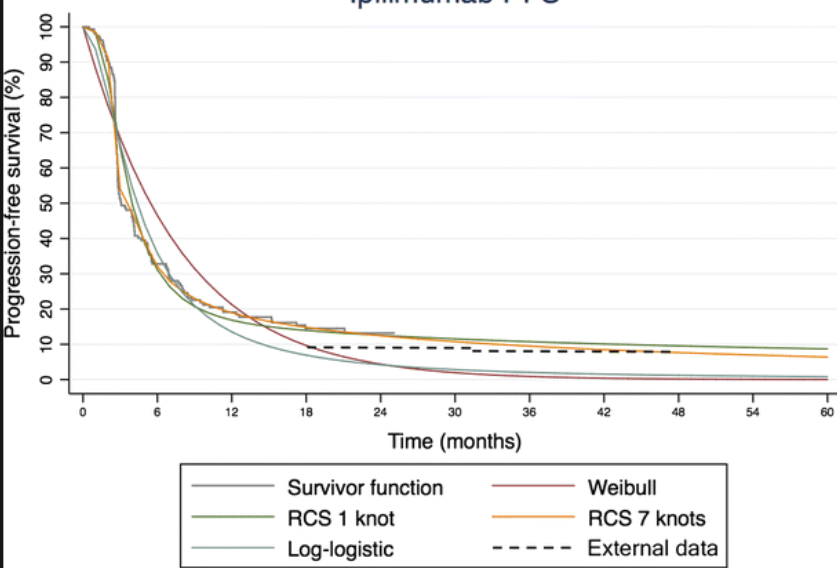
\includegraphics[width=1\linewidth]{figures/flexsurv}

\end{frame}

\begin{frame}{Spline Survival models}
\protect\hypertarget{spline-survival-models-2}{}

From Gibson et al (Pharacoeconomcs, 2017)

\emph{Spline-based models using a limited number of knots can provide an
acceptable fit to trial data and generate extrapolated estimates
supported by longer term evidence, with results that are stable in
response to changes in knot placement.}

\end{frame}

\begin{frame}{Approaches in extrapolation}
\protect\hypertarget{approaches-in-extrapolation}{}

Modeler faced with a more decisions: - Extrapolate using KM and
``fitted'' tails - Extrapolate using the fitted curve

\begin{itemize}
\tightlist
\item
  Fit seperate curves to the data
\item
  Extrapolate treatment effect as relative
\item
  What is the behaviour of the relative effect post trial?
\end{itemize}

\end{frame}

\begin{frame}{Approaches in extrapolation}
\protect\hypertarget{approaches-in-extrapolation-1}{}


\includegraphics[width=1\linewidth]{figures/endmeans}

\end{frame}

\begin{frame}{Approaches in extrapolation}
\protect\hypertarget{approaches-in-extrapolation-2}{}

\begin{itemize}
\tightlist
\item
  Extrapolate using KM and ``fitted'' tails
\end{itemize}

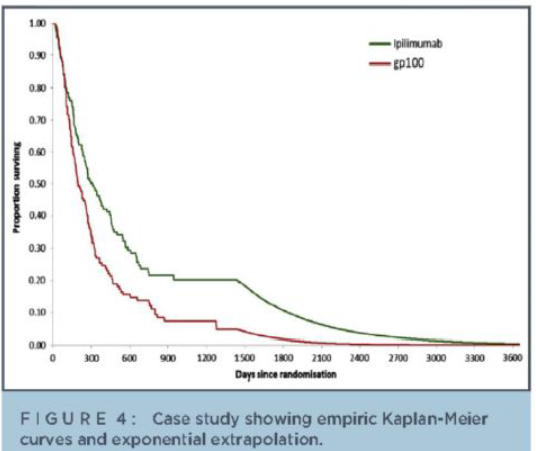
\includegraphics[width=1\linewidth]{figures/figure4means}

\end{frame}

\begin{frame}

\begin{itemize}
\tightlist
\item
  Extrapolate using the fitted curve
\end{itemize}

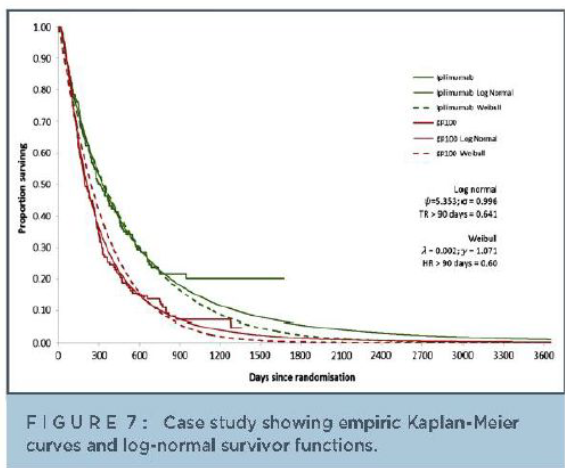
\includegraphics[width=1\linewidth]{figures/figure7means}

\end{frame}

\begin{frame}{Extrapolating a relative treatment effect}
\protect\hypertarget{extrapolating-a-relative-treatment-effect}{}

Drummond, et al (2015). Methods for the economic evaluation of health
care programmes. Oxford university press.

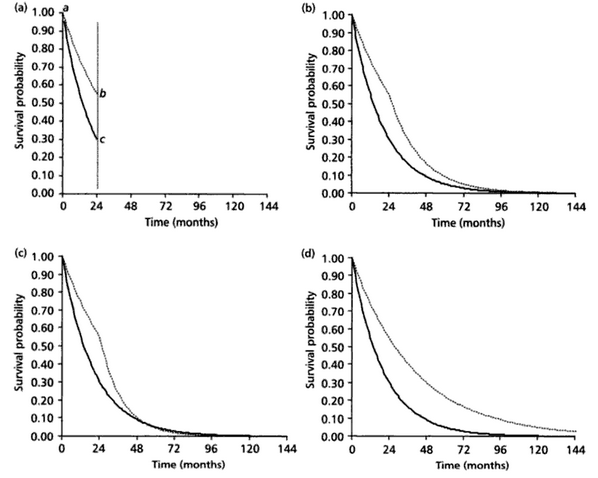
\includegraphics[width=0.8\linewidth]{figures/drummond}

\end{frame}

\begin{frame}{Partitioned survival models}
\protect\hypertarget{partitioned-survival-models}{}

\begin{itemize}
\tightlist
\item
  Form of a decision model that:

  \begin{itemize}
  \tightlist
  \item
    Considers evidence of (usually) OS and PFS
  \item
    allocates the cohort across pre-progression, post-progression, death
  \end{itemize}
\item
  PFS and OS are modeled independently
\end{itemize}

\end{frame}

\begin{frame}

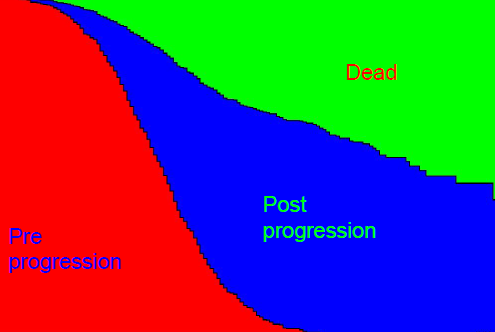
\includegraphics[width=1\linewidth]{figures/psm}

\end{frame}

\begin{frame}{Partitioned survival models}
\protect\hypertarget{partitioned-survival-models-1}{}

\begin{itemize}
\tightlist
\item
  Mechanics:

  \begin{itemize}
  \tightlist
  \item
    Remain pre-progression: p(PFS)
  \item
    Remain dead: 1 -- p(OS)
  \item
    Progressed: p(OS) - p(PFS)
  \end{itemize}
\item
  Implicit assumption: risk of dying is only a function of time
\end{itemize}

\end{frame}

\begin{frame}

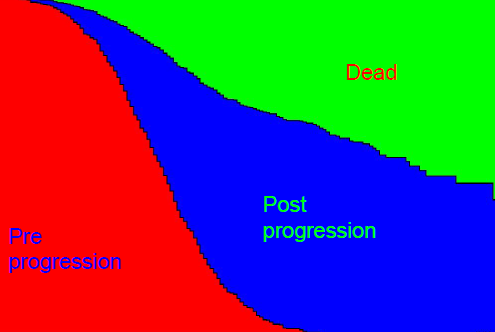
\includegraphics[width=1\linewidth]{figures/psm}

Less problematic with less censoring

\end{frame}

\begin{frame}{Partitioned survival models - the updside}
\protect\hypertarget{partitioned-survival-models---the-updside}{}

\begin{itemize}
\tightlist
\item
  Intuitively appealing
\item
  Easy to communicate
\item
  Easy to construct
\item
  In-sync with what is commonly reported in RCTs
\item
  Can be constructed using aggregate / graphic based data
\item
  In-sync with methods of cross-over
\item
  PSMs work great for cases where the whole cohort is observed until
  event of interest (unlikely in the vast majority of the cases)
\end{itemize}

\end{frame}

\begin{frame}{Partitioned survival models - the downside}
\protect\hypertarget{partitioned-survival-models---the-downside}{}

\begin{itemize}
\tightlist
\item
  OS and PFS are falsely assumed independent
\item
  Cohort cannot transition back to a healthier state.
\item
  3-state PSM cannot distinguish the origin of the cohort moving to the
  dead state (progresed -\textgreater{} death vs preprogession
  -\textgreater{} death)
\item
  In the presence of censoring:

  \begin{itemize}
  \tightlist
  \item
    Projected trajectory of state occupancy after end of follow up only
    informed by the observed trajectory
  \item
    Poor performance when trends in the within trial period may not
    continue in the extrapolation period
  \end{itemize}
\end{itemize}

\end{frame}

\begin{frame}{Partitioned survival models - the criticism}
\protect\hypertarget{partitioned-survival-models---the-criticism}{}

Woods et al 2017 (DSU 19)


\includegraphics[width=1\linewidth]{figures/psmcritic}

\end{frame}

\begin{frame}

Williams et al 2017 (MDM)

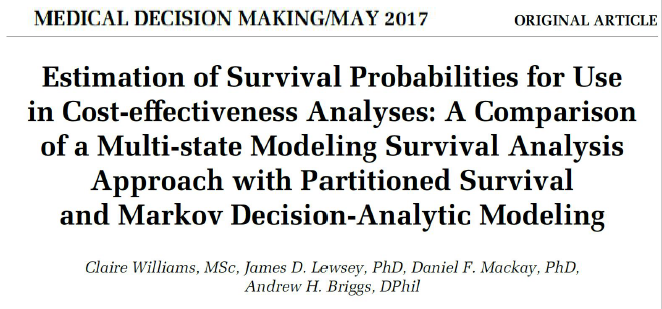
\includegraphics[width=1\linewidth]{figures/williams2017}

\end{frame}

\begin{frame}{Competing Risks}
\protect\hypertarget{competing-risks}{}

\begin{itemize}
\tightlist
\item
  Underlying assumption in survival analysis:

  \begin{itemize}
  \tightlist
  \item
    If we could follow censored individuals long enough they would
    experience the event of interest.
  \end{itemize}
\item
  Event B (progression) affecs population size at risk for the competing
  event C
\end{itemize}

\end{frame}

\begin{frame}

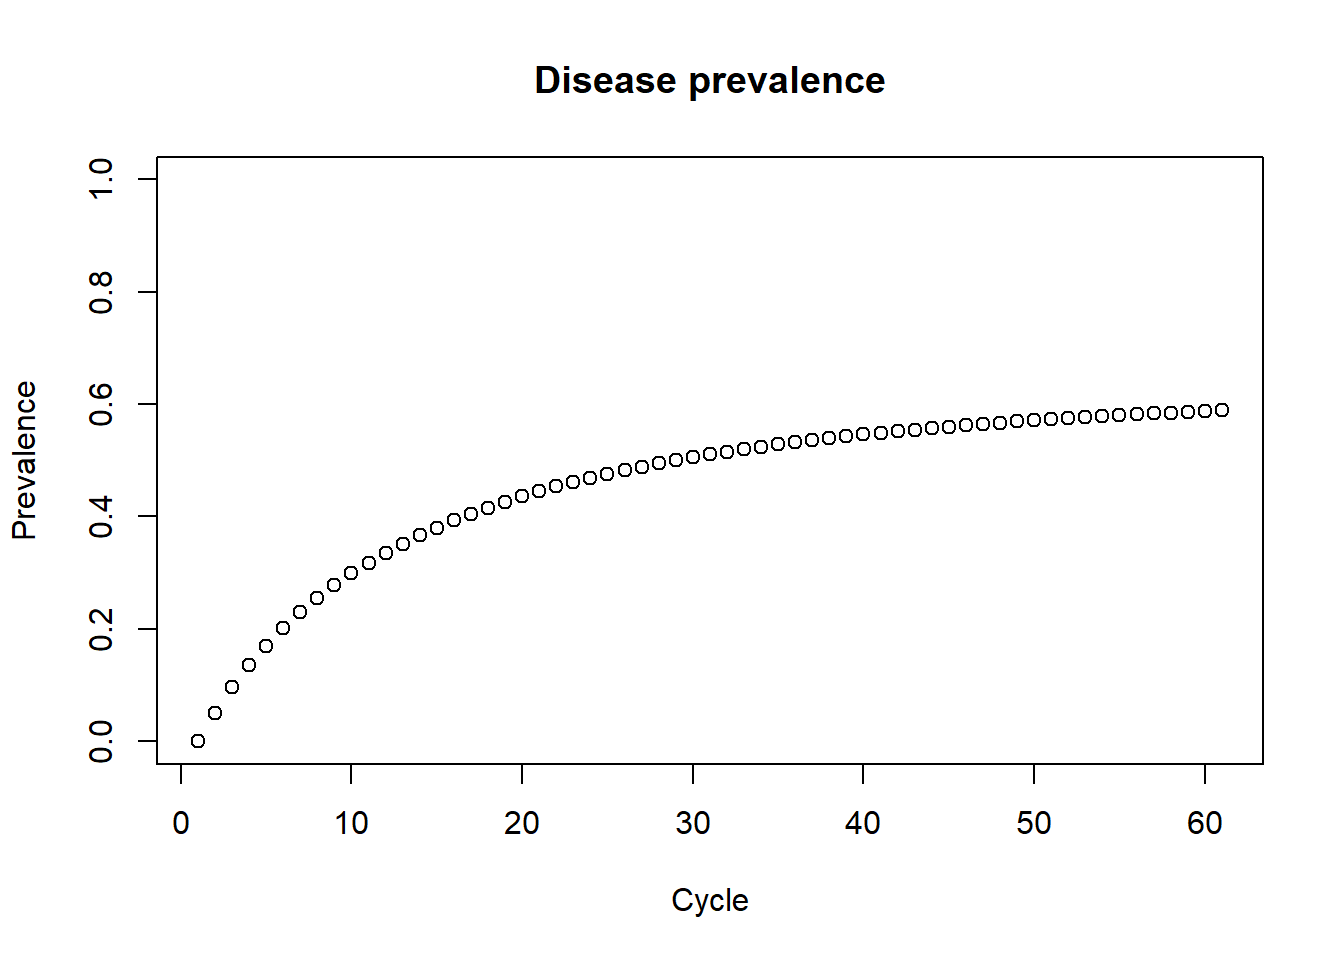
\includegraphics{SMDM_surv_files/figure-beamer/unnamed-chunk-15-1.pdf}

\end{frame}

\begin{frame}{Multistate modeling}
\protect\hypertarget{multistate-modeling}{}

\begin{itemize}
\tightlist
\item
  Extended form of competing risks
\item
  Multivariate survival analysis
\end{itemize}

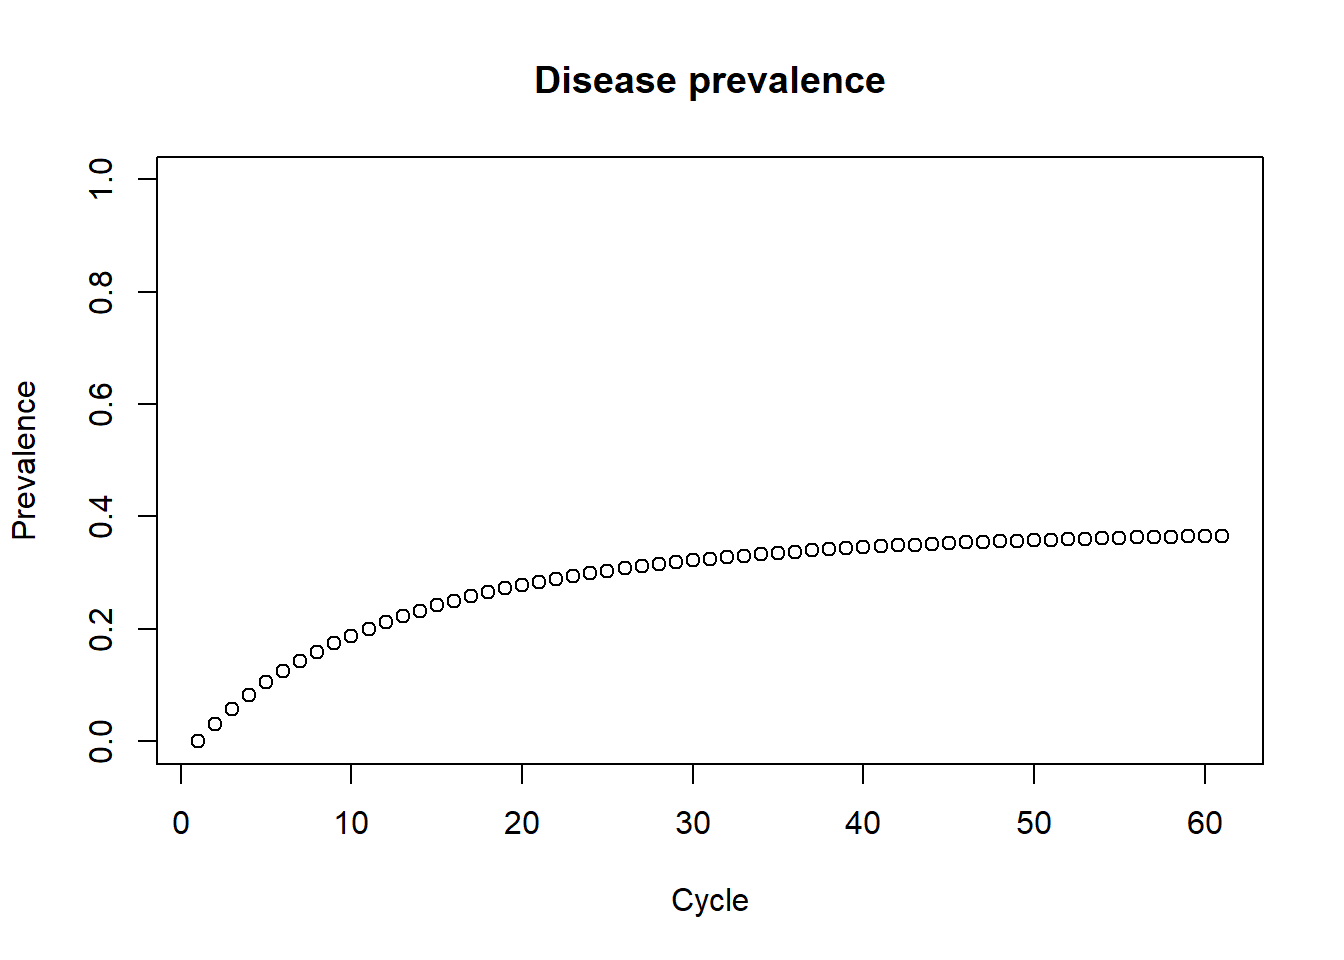
\includegraphics{SMDM_surv_files/figure-beamer/unnamed-chunk-16-1.pdf}

\end{frame}

\begin{frame}{Multistate modeling}
\protect\hypertarget{multistate-modeling-1}{}

\begin{itemize}
\tightlist
\item
  Extended form of competing risks
\item
  Multivariate survival analysis
\item
  Can incorporate:

  \begin{itemize}
  \tightlist
  \item
    Transition specific covariates
  \item
    Recurrent events
  \end{itemize}
\item
  Can work with

  \begin{itemize}
  \tightlist
  \item
    Patient-level data (best)
  \item
    Digitized / interval censored data (\ldots{}not best)
  \end{itemize}
\end{itemize}

\end{frame}

\begin{frame}[fragile]{Multistate modeling}
\protect\hypertarget{multistate-modeling-2}{}

Fitted in two ways:

\begin{enumerate}
\tightlist
\item
  separate models for each trasition
\end{enumerate}

\begin{itemize}
\tightlist
\item
  recurrent events
\item
  covariates
\item
  seperate dataset for each (non-saturating) state
\item
  ``naive'' assumption of censoring when competing event occurs
\item
  easy to fit in R \texttt{flexsurv} and \texttt{mstate}
\end{itemize}

\end{frame}

\begin{frame}[fragile]{Multistate modeling}
\protect\hypertarget{multistate-modeling-3}{}

Fitted in two ways:

\begin{enumerate}
\setcounter{enumi}{1}
\tightlist
\item
  Joint multivariate model for all transitions - Powerfull!

  \begin{itemize}
  \tightlist
  \item
    Mislclassification errors
  \item
    Latent states
  \item
    Interval censoring
  \item
    Continuous time
  \end{itemize}
\end{enumerate}

Drawbacks: - Difficult to converge - Limited options wrt assumed
distributions (exponential)

Can be fitted through \texttt{msm} and \texttt{flexsurv}

\end{frame}

\begin{frame}{Multistate modeling}
\protect\hypertarget{multistate-modeling-4}{}

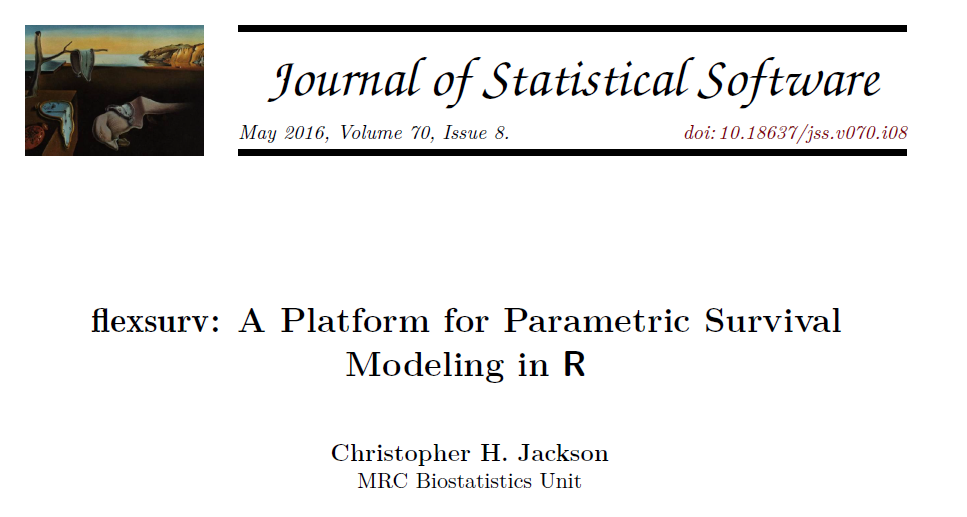
\includegraphics[width=1\linewidth]{figures/jacksonflex}

Great resource for both survival fitting and multistate models

\end{frame}

\begin{frame}{Multistate \& microsimulation}
\protect\hypertarget{multistate-microsimulation}{}

\begin{itemize}
\tightlist
\item
  Multistate models allow for time-dependent transition probabilities
\item
  When dependence on time-in-state partioned survival / markov models
  are inadequate\\
\item
  Necessary solution: Individual level simulation modeling
\end{itemize}

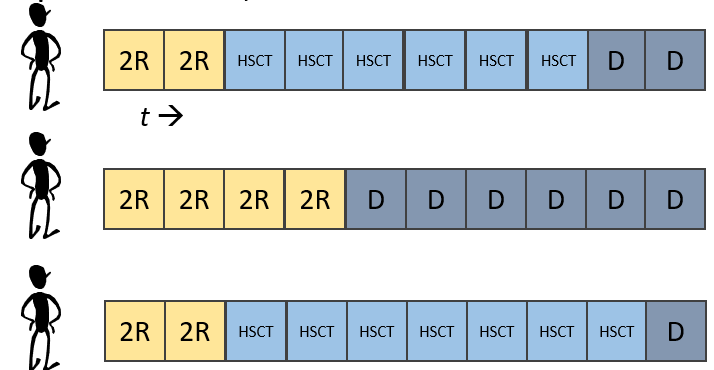
\includegraphics[width=1\linewidth]{figures/microsim}

\end{frame}

\begin{frame}{Multistate modeling}
\protect\hypertarget{multistate-modeling-5}{}

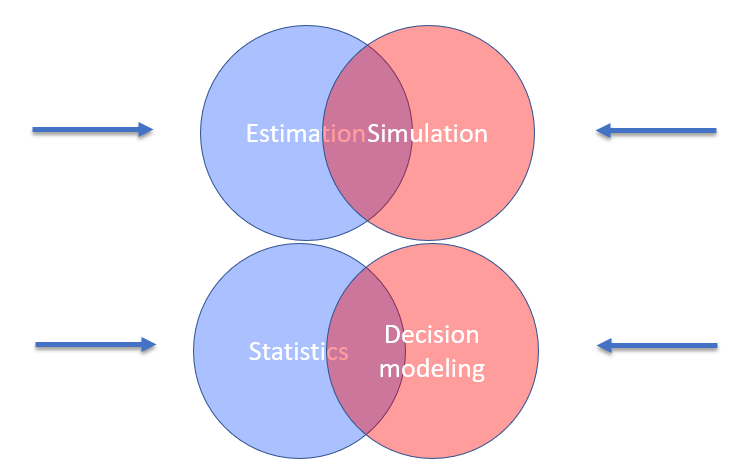
\includegraphics[width=1\linewidth]{figures/venn}

\end{frame}

\begin{frame}{Multistate modeling}
\protect\hypertarget{multistate-modeling-6}{}


\includegraphics[width=0.8\linewidth]{figures/msmnice}

\end{frame}

\begin{frame}{External data and survival models}
\protect\hypertarget{external-data-and-survival-models}{}

Given short term follow up in RCTs, survival extrapolations can be
informed by external data

\begin{itemize}
\tightlist
\item
  Adjustment of all-cause mortality using life-tables
\item
  Expert opinion on plausibility
\end{itemize}

Other sources of external data:

\begin{itemize}
\tightlist
\item
  longer follow-up on a different RCT
\item
  disease registry
\item
  administrative data
\end{itemize}

\end{frame}

\begin{frame}{External data and survival models}
\protect\hypertarget{external-data-and-survival-models-1}{}

Observational data

\begin{itemize}
\tightlist
\item
  possibly more representative of the real world
\item
  at risk for (unmeasured) confounding
\end{itemize}

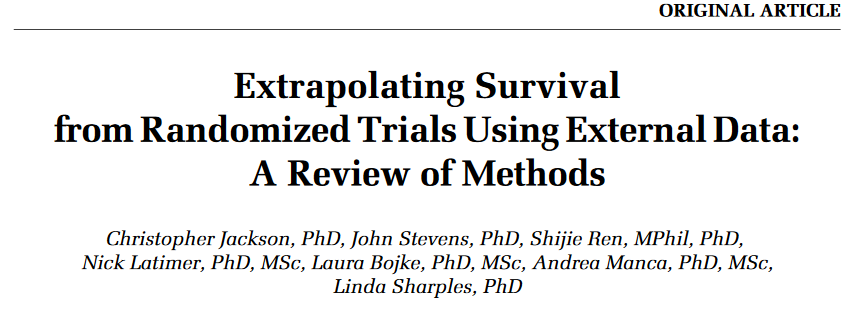
\includegraphics[width=1\linewidth]{figures/jacksonext}

\end{frame}

\begin{frame}{External data and survival models}
\protect\hypertarget{external-data-and-survival-models-2}{}

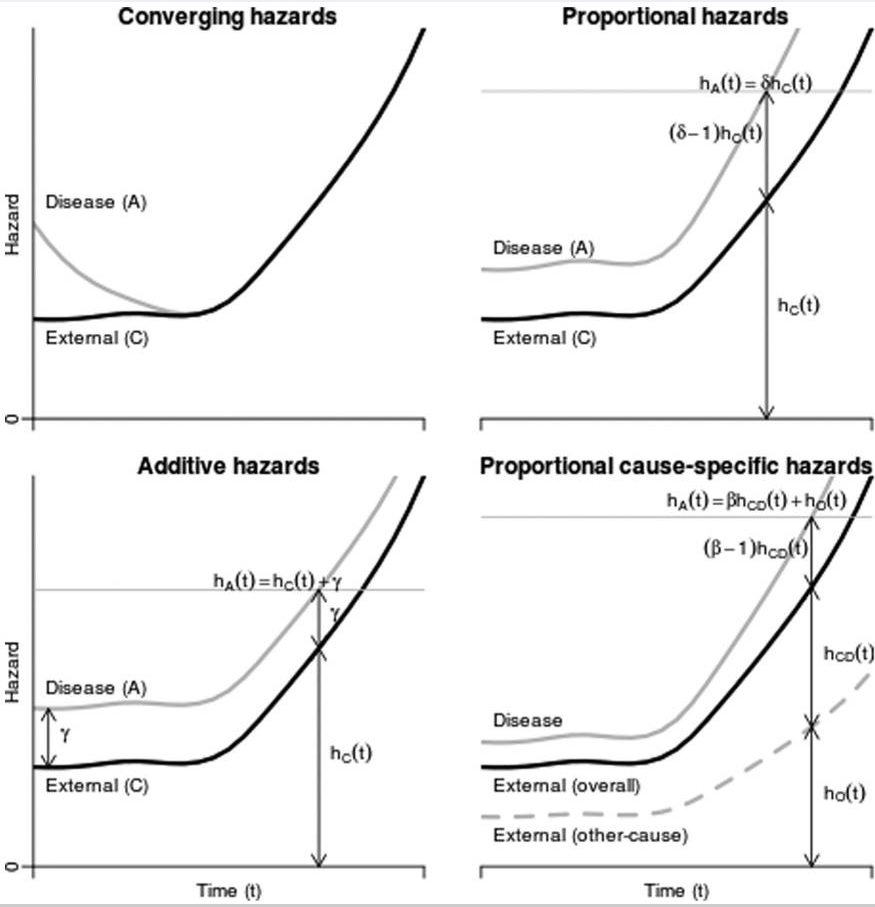
\includegraphics[width=0.7\linewidth]{figures/jacksonfig3}

\end{frame}

\begin{frame}{Mixture Cure Models - Main Points}
\protect\hypertarget{mixture-cure-models---main-points}{}

\begin{itemize}
\tightlist
\item
  Therapies with the possibility of cure pose a modeling challenge
\item
  e.g.~plateau on immotherapy survival curves
\item
  Extrapolation challenging without external information
\item
  Traditional methods: Underestimation more likely than over estimation
  of the effect
\end{itemize}

\end{frame}

\begin{frame}{Mixture Cure Models - Main Points}
\protect\hypertarget{mixture-cure-models---main-points-1}{}

\begin{itemize}
\tightlist
\item
  extension of survival models where a proportion of the population is
  assumed to be ``cured''

  \begin{itemize}
  \tightlist
  \item
    non-cured fraction at risk of progression and death informed by the
    trial
  \item
    cured fraction at risk of death informed by external data.
  \end{itemize}
\end{itemize}

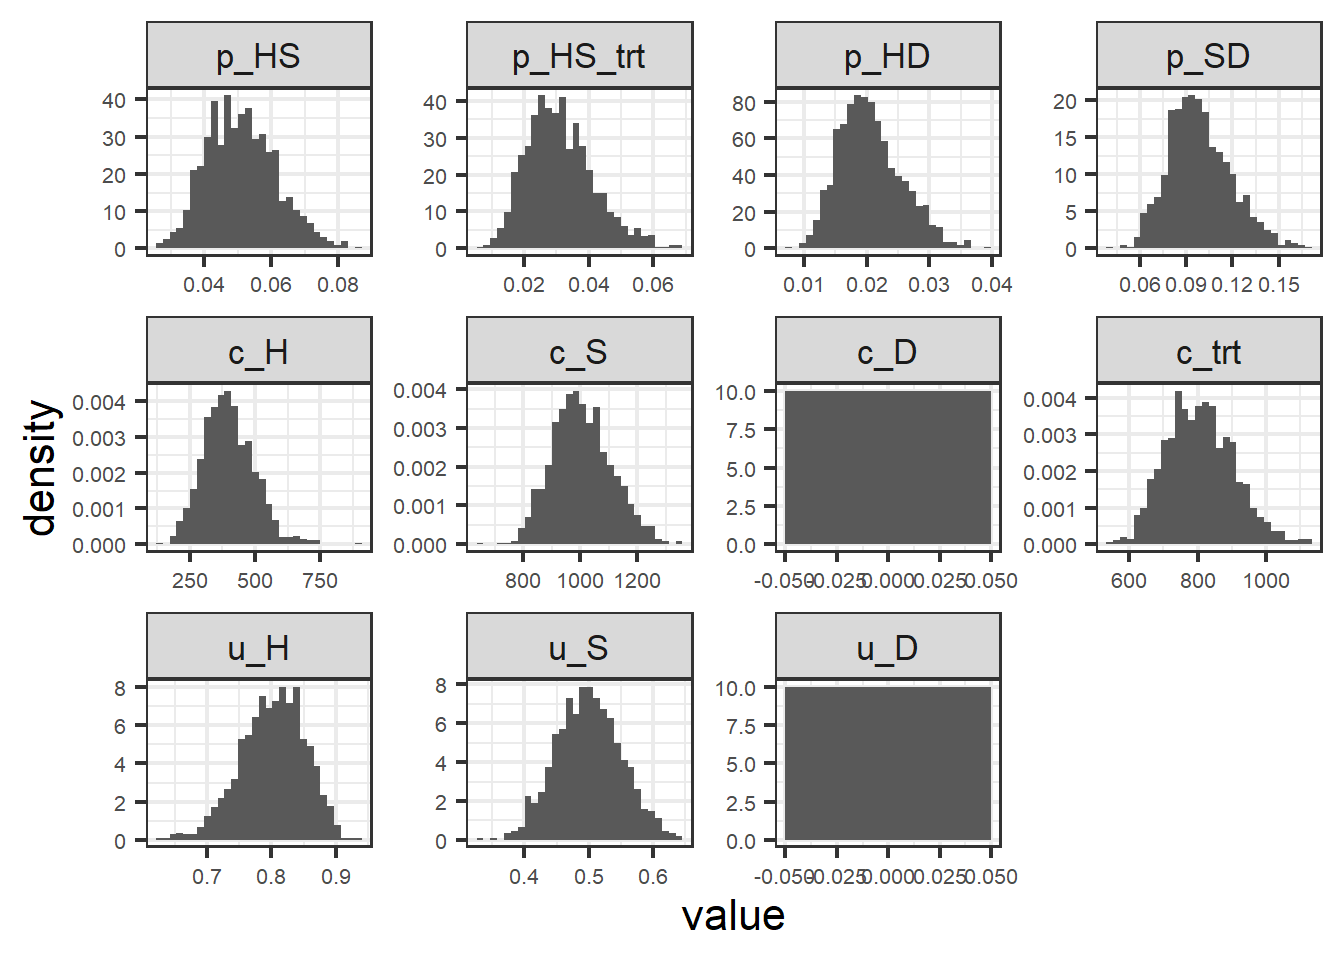
\includegraphics[width=0.85\linewidth]{SMDM_surv_files/figure-beamer/unnamed-chunk-23-1}

\end{frame}

\begin{frame}{Mixture Cure Models - Estimation}
\protect\hypertarget{mixture-cure-models---estimation}{}

\begin{itemize}
\item
  Cure rate models a promising solution but the cure faction difficult
  to estimate
\item
  Can be fitted in both R and SAS
\item
  Guidance is lacking but given the popularity soon to come!
\end{itemize}

\end{frame}

\begin{frame}{Mixture Cure Models - Validity}
\protect\hypertarget{mixture-cure-models---validity}{}

\begin{itemize}
\tightlist
\item
  Paucity of applications in HTA
\end{itemize}


\includegraphics[width=1\linewidth]{figures/latimercure}

\begin{itemize}
\tightlist
\item
  Recently shown to be more appropriate than conventional modeling (n of
  1)
\end{itemize}

\end{frame}

\begin{frame}{Thank you!}
\protect\hypertarget{thank-you}{}

\end{frame}

\end{document}
